% Supplement to the merged manuscript (paper1 + paper3) prepared for the Journal of Medical Imaging (SPIE), following the
% SPIE journal manuscript guidelines (structured abstract, 3-6 keywords, Times 12 pt, US letter, 1 in margins,
% superscript numbered citations in order of first citation, DOIs in brackets).
% The official class spieman.cls is not installed locally, so the specified formatting is reproduced with
% standard packages; swap in spieman.cls at submission time if the journal portal requires it.
%
% TODO(author): confirm the abstract word limit and any JMI-specific items on the journal's author guidelines page.
% TODO(author): add co-authors/supervisor if any (currently sole author), and any other AI tools used in the study
%               (code, figures) to the Materials and Methods section on generative AI use.
% TODO(author): confirm the Disclosures wording and the code-availability choice (repository is currently private).
% TODO(author): fill exact software versions and the latency-laptop CPU model/threads in the reproducibility table (Table 'tab:repro').
% TODO(author): consider a cluster-level re-split and bootstrap CIs (needs retraining/re-inference); see Limitations.
\documentclass[12pt,letterpaper]{article}
\usepackage[letterpaper,margin=1in]{geometry}
\usepackage{mathptmx}
\usepackage{graphicx}
\usepackage{booktabs}
\usepackage{amsmath}
\usepackage{url}
\usepackage{setspace}
\usepackage[super,comma,sort&compress]{natbib}
\usepackage{titlesec}
\titleformat{\section}{\fontsize{12}{14}\selectfont\bfseries}{\thesection}{1em}{}
\titleformat{\subsection}{\fontsize{12}{14}\selectfont\itshape}{\thesubsection}{1em}{}
\titleformat{\subsubsection}{\fontsize{11}{13}\selectfont\itshape}{\thesubsubsection}{1em}{}
\setlength{\parindent}{0.2in}
\setstretch{1.15}
\renewcommand{\bibnumfmt}[1]{#1.}
\setlength{\bibsep}{2pt}

\begin{document}
\begin{flushleft}
{\fontsize{14}{17}\selectfont\bfseries Supplementary material: trustworthiness is not one property in single-cell cervical cytology classification\par}
\vspace{8pt}
{\fontsize{11}{13}\selectfont Md. Mostafizur Rahman, San Francisco Bay University\par}
\end{flushleft}

\renewcommand{\thetable}{S\arabic{table}}
\renewcommand{\thefigure}{S\arabic{figure}}

This supplement holds tables and figures referenced in the main manuscript as Tables S1--S10 and Figures S1--S6. Section numbers refer to the main manuscript.

\begin{table}[htbp]
\centering
\caption{In-distribution benchmark on SIPaKMeD, all 12 models, sorted by balanced accuracy (seed 13).}
\label{tab:bench}
\begin{tabular}{lrrrr}
\toprule
Model & Bal.\ acc. & Macro F1 & AUROC & Params \\
\midrule
\textbf{EfficientViT-M0} & \textbf{0.9654} & \textbf{0.9656} & 0.9985 & \textbf{2{,}157{,}401} \\
EfficientViT-B0 & 0.9623 & 0.9624 & 0.9983 & 2{,}135{,}413 \\
DeiT-Tiny & 0.9606 & 0.9607 & 0.9974 & 5{,}525{,}381 \\
Swin-Tiny & 0.9605 & 0.9606 & 0.9965 & 27{,}523{,}199 \\
TinyViT-5M & 0.9587 & 0.9589 & 0.9979 & 5{,}073{,}369 \\
MobileViT-S & 0.9570 & 0.9575 & 0.9979 & 4{,}940{,}837 \\
ResNet-50 & 0.9542 & 0.9540 & 0.9966 & 23{,}518{,}277 \\
LeViT-128 & 0.9458 & 0.9456 & 0.9946 & 8{,}447{,}786 \\
MobileViTv2 & 0.9387 & 0.9401 & 0.9966 & 4{,}391{,}406 \\
EfficientNet-Lite0 & 0.9375 & 0.9376 & 0.9944 & 3{,}377{,}413 \\
ViT-Small & 0.9374 & 0.9380 & 0.9960 & 21{,}667{,}589 \\
MobileNetV2 & 0.9357 & 0.9365 & 0.9952 & 2{,}230{,}277 \\
\bottomrule
\end{tabular}
\end{table}

\begin{table}[htbp]
\centering
\caption{Balanced accuracy of all 12 models, seed 13, sorted by Mendeley LBC score. The SIPaKMeD column is five-class in-distribution balanced accuracy from the same run (chance 0.20); the Herlev and Mendeley LBC columns are zero-shot binary normal/abnormal balanced accuracy (chance 0.50). The scales are not comparable, so only ranks are compared across columns.}
\label{tab:shift12}
\small
\begin{tabular}{lrrr}
\toprule
Model (family, params) & SIPaKMeD (5-class) & Herlev & Mendeley LBC \\
\midrule
EfficientNet-Lite0 (CNN, 3.38M) & 0.9455 & 0.5970 & \textbf{0.6674} \\
ResNet-50 (CNN, 23.5M) & 0.9556 & 0.6838 & 0.6082 \\
MobileViTv2 (eff.\ ViT, 4.39M) & 0.9638 & \textbf{0.7501} & 0.5418 \\
MobileNetV2 (CNN, 2.23M) & 0.9505 & 0.6919 & 0.5391 \\
DeiT-Tiny (eff.\ ViT, 5.5M) & 0.9504 & 0.7151 & 0.5230 \\
EfficientViT-B0 (eff.\ ViT, 2.14M) & 0.9738 & 0.6818 & 0.5217 \\
Swin-Tiny (full ViT, 27.5M) & 0.9590 & 0.7282 & 0.5192 \\
ViT-Small (full ViT, 21.7M) & 0.9573 & 0.7049 & 0.5084 \\
LeViT-128 (eff.\ ViT, 8.4M) & 0.9526 & 0.5777 & 0.4764 \\
EfficientViT-M0 (eff.\ ViT, 2.16M) & 0.9737 & 0.6716 & 0.4731 \\
TinyViT-5M (eff.\ ViT, 5.1M) & 0.9685 & 0.7327 & 0.4543 \\
MobileViT-S (eff.\ ViT, 4.94M) & 0.9520 & 0.7104 & \textbf{0.2927} (AUROC 0.215) \\
\bottomrule
\end{tabular}
\end{table}

\begin{table}[htbp]
\centering
\caption{Zero-shot binary evaluation of all 12 models on APCEM, sorted by AUROC. This table comes from a separate training run, so the five-class in-distribution balanced accuracy in the SIPaKMeD column differs from Table~S2.}
\label{tab:apcem}
\small
\begin{tabular}{lrrr}
\toprule
Model (family, params) & SIPaKMeD (5-class) & APCEM bal.\ acc. & APCEM AUROC \\
\midrule
MobileNetV2 (CNN, 2.23M) & 0.9623 & \textbf{0.6158} & \textbf{0.6528} \\
EfficientNet-Lite0 (CNN, 3.38M) & 0.9309 & 0.5393 & 0.5701 \\
LeViT-128 (eff.\ ViT, 8.4M) & 0.9001 & 0.5263 & 0.5376 \\
Swin-Tiny (full ViT, 27.5M) & 0.9330 & 0.4724 & 0.3082 \\
EfficientViT-B0 (eff.\ ViT, 2.14M) & 0.9638 & 0.4481 & 0.3206 \\
DeiT-Tiny (eff.\ ViT, 5.5M) & 0.9589 & 0.4469 & 0.3799 \\
MobileViTv2 (eff.\ ViT, 4.39M) & 0.9570 & 0.4290 & 0.4120 \\
TinyViT-5M (eff.\ ViT, 5.1M) & 0.9670 & 0.4100 & 0.3681 \\
EfficientViT-M0 (eff.\ ViT, 2.16M) & 0.9621 & 0.3730 & 0.3407 \\
MobileViT-S (eff.\ ViT, 4.94M) & 0.9687 & 0.3621 & 0.3161 \\
ViT-Small (full ViT, 21.7M) & 0.9538 & 0.3444 & 0.2555 \\
ResNet-50 (CNN, 23.5M) & 0.9639 & \textbf{0.3339} & 0.2929 \\
\bottomrule
\end{tabular}
\end{table}

\begin{table}[htbp]
\centering
\caption{Mean $\pm$ standard deviation of balanced accuracy over three training seeds (13, 17, 29), in the row order of Table~S2. The SIPaKMeD column is five-class; the external columns are binary. Seed 13 values are those of Tables~S2 and~S3, which come from separate runs.}
\label{tab:seeds}
\footnotesize
\begin{tabular}{lrrrr}
\toprule
Model & SIPaKMeD (5-class) & Herlev & Mendeley LBC & APCEM \\
\midrule
EfficientNet-Lite0 & 0.951 $\pm$ 0.006 & 0.630 $\pm$ 0.030 & 0.630 $\pm$ 0.106 & 0.544 $\pm$ 0.027 \\
ResNet-50 & 0.957 $\pm$ 0.002 & 0.689 $\pm$ 0.005 & 0.537 $\pm$ 0.062 & 0.390 $\pm$ 0.072 \\
MobileViTv2 & 0.964 $\pm$ 0.004 & 0.721 $\pm$ 0.025 & 0.516 $\pm$ 0.064 & 0.466 $\pm$ 0.033 \\
MobileNetV2 & 0.946 $\pm$ 0.004 & 0.659 $\pm$ 0.030 & 0.563 $\pm$ 0.083 & 0.586 $\pm$ 0.026 \\
DeiT-Tiny & 0.955 $\pm$ 0.004 & 0.700 $\pm$ 0.015 & 0.484 $\pm$ 0.036 & 0.385 $\pm$ 0.059 \\
EfficientViT-B0 & 0.966 $\pm$ 0.008 & 0.667 $\pm$ 0.017 & 0.575 $\pm$ 0.047 & 0.442 $\pm$ 0.035 \\
Swin-Tiny & 0.961 $\pm$ 0.005 & 0.720 $\pm$ 0.009 & 0.481 $\pm$ 0.034 & 0.419 $\pm$ 0.047 \\
ViT-Small & 0.957 $\pm$ 0.008 & 0.705 $\pm$ 0.048 & 0.477 $\pm$ 0.055 & 0.392 $\pm$ 0.045 \\
LeViT-128 & 0.900 $\pm$ 0.065 & 0.538 $\pm$ 0.034 & 0.507 $\pm$ 0.031 & 0.518 $\pm$ 0.016 \\
EfficientViT-M0 & 0.966 $\pm$ 0.009 & 0.681 $\pm$ 0.015 & 0.502 $\pm$ 0.038 & 0.409 $\pm$ 0.043 \\
TinyViT-5M & 0.968 $\pm$ 0.001 & 0.706 $\pm$ 0.025 & 0.453 $\pm$ 0.010 & 0.422 $\pm$ 0.018 \\
MobileViT-S & 0.958 $\pm$ 0.005 & 0.689 $\pm$ 0.029 & 0.387 $\pm$ 0.084 & 0.372 $\pm$ 0.024 \\
\bottomrule
\end{tabular}
\end{table}

\begin{table}[htbp]
\centering
\caption{Parameters, FLOPs (multiply-add counted as 2), and median single-image CPU latency for all 12 models (untrained weights, one shared consumer laptop).}
\label{tab:eff}
\small
\begin{tabular}{lrrr}
\toprule
Model & Params & FLOPs (G) & CPU latency (ms) \\
\midrule
EfficientViT-M0 & 2{,}157{,}401 & 0.158 & 36.2 \\
EfficientViT-B0 & 2{,}135{,}413 & 0.198 & 41.6 \\
MobileNetV2 & 2{,}230{,}277 & 0.599 & 33.5 \\
EfficientNet-Lite0 & 3{,}377{,}413 & 0.768 & \textbf{137.7} \\
LeViT-128 & 8{,}447{,}786 & 0.809 & 17.5 \\
DeiT-Tiny & 5{,}525{,}381 & 2.149 & \textbf{15.4} \\
TinyViT-5M & 5{,}073{,}369 & 2.510 & 44.9 \\
MobileViT-S & 4{,}940{,}837 & 3.645 & 66.3 \\
MobileViTv2 & 4{,}391{,}406 & 3.623 & 65.2 \\
ResNet-50 & 23{,}518{,}277 & 8.174 & 32.0 \\
ViT-Small & 21{,}667{,}589 & 8.482 & 26.8 \\
Swin-Tiny & 27{,}523{,}199 & 8.980 & 54.0 \\
\bottomrule
\end{tabular}
\end{table}

\begin{table}[htbp]
\centering
\caption{Explainability scores on all 596 cluster-grouped test cells, mean [95\% cluster-bootstrap interval]. Lower is better for deletion AUC, and higher is better for insertion AUC and nucleus concentration (1.0 is chance).}
\label{tab:xai-full}
\footnotesize
\begin{tabular}{@{}llccc@{}}
\toprule
Backbone & Method & Deletion AUC & Insertion AUC & Nucleus concentration \\
\midrule
DeiT-Tiny & Relevancy propagation & 0.727 [0.678, 0.777] & 0.966 [0.957, 0.973] & 3.79 [2.80, 4.81] \\
DeiT-Tiny & Attention rollout & 0.807 [0.768, 0.845] & 0.941 [0.925, 0.955] & 1.35 [1.15, 1.59] \\
DeiT-Tiny & Grad-CAM & 0.816 [0.779, 0.852] & 0.904 [0.876, 0.931] & 1.19 [1.01, 1.37] \\
\addlinespace
ViT-Small & Relevancy propagation & 0.721 [0.653, 0.789] & 0.961 [0.952, 0.970] & 4.79 [3.49, 6.17] \\
ViT-Small & Attention rollout & 0.766 [0.699, 0.831] & 0.947 [0.932, 0.959] & 1.95 [1.69, 2.22] \\
ViT-Small & Grad-CAM & 0.910 [0.886, 0.931] & 0.780 [0.714, 0.843] & 1.17 [0.91, 1.43] \\
\bottomrule
\end{tabular}
\end{table}

\begin{table}[htbp]
\centering
\caption{Explainability method comparison on DeiT-Tiny, 50 SIPaKMeD test images (10 per class), all matched to a real nucleus polygon.}
\label{tab:xai}
\begin{tabular}{lrrr}
\toprule
Method & Deletion AUC$\downarrow$ & Insertion AUC$\uparrow$ & Nucleus conc.$\uparrow$ \\
\midrule
\textbf{Relevancy propagation} & \textbf{0.734} & \textbf{0.970} & \textbf{2.714} \\
Grad-CAM (ViT-adapted) & 0.818 & 0.877 & 1.472 \\
Attention rollout & 0.825 & 0.936 & 1.177 \\
\bottomrule
\end{tabular}
\end{table}

\begin{table}[htbp]
\centering
\caption{Explainability ranking on a second backbone (ViT-Small) versus the original (DeiT-Tiny).}
\label{tab:xai-vits}
\small
\begin{tabular}{lrrrrrr}
\toprule
 & \multicolumn{3}{c}{DeiT-Tiny (original)} & \multicolumn{3}{c}{ViT-Small (2nd backbone)} \\
Method & Del.$\downarrow$ & Ins.$\uparrow$ & Conc.$\uparrow$ & Del.$\downarrow$ & Ins.$\uparrow$ & Conc.$\uparrow$ \\
\midrule
\textbf{Relevancy prop.} & \textbf{0.734} & \textbf{0.970} & \textbf{2.71} & \textbf{0.816} & \textbf{0.965} & \textbf{4.20} \\
Grad-CAM & 0.818 & 0.877 & 1.47 & 0.888 & 0.895 & 1.35 \\
Attn.\ rollout & 0.825 & 0.936 & 1.18 & 0.888 & 0.927 & 0.97 \\
\bottomrule
\end{tabular}
\end{table}

\begin{figure}[htbp]
\centering
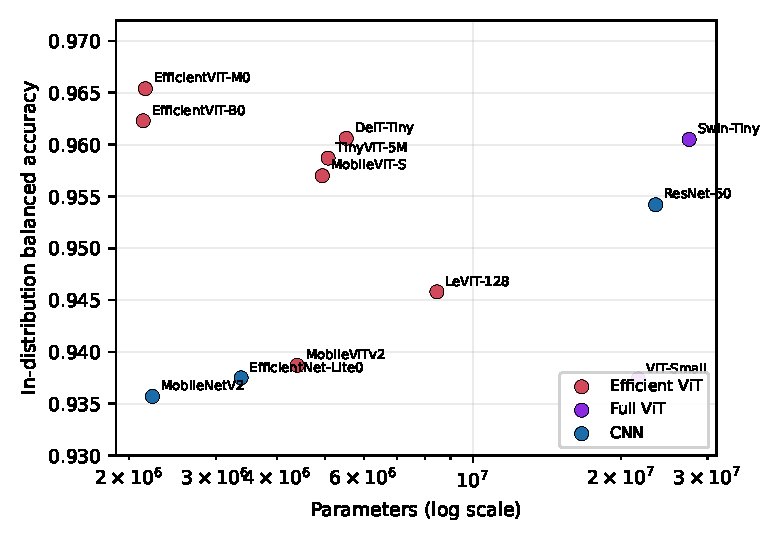
\includegraphics[width=0.82\textwidth]{figs/p1_fig1_params_vs_accuracy.pdf}
\caption{Parameters (log scale) versus in-distribution balanced accuracy, colored by architecture family. The two efficient-ViT models with the fewest parameters (EfficientViT-M0 and -B0) are also the two most accurate in this run.}
\label{fig:params-vs-acc}
\end{figure}

\begin{figure}[htbp]
\centering
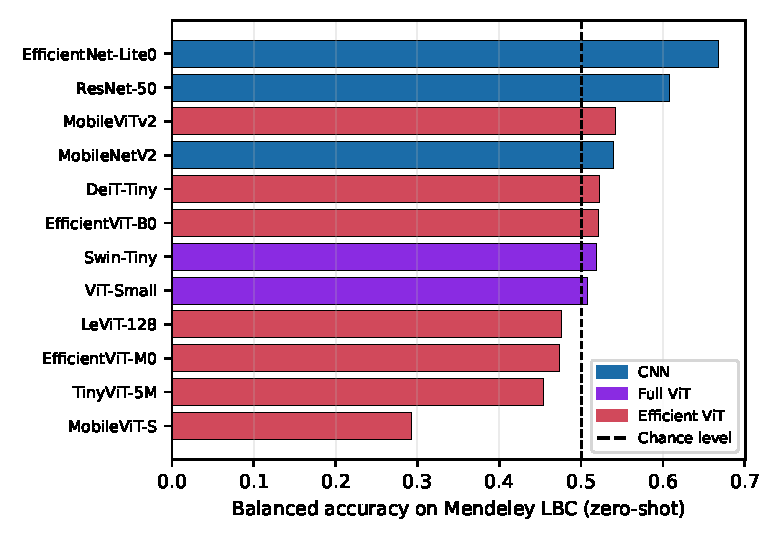
\includegraphics[width=0.82\textwidth]{figs/p1_fig2_mendeley_shift.pdf}
\caption{Balanced accuracy on Mendeley LBC (zero-shot), sorted and colored by architecture family. All three CNNs cluster above chance, and eight of nine transformer-family models cluster at or below chance, with MobileViT-S the sole catastrophic outlier.}
\label{fig:mendeley-shift}
\end{figure}

\begin{figure}[htbp]
\centering
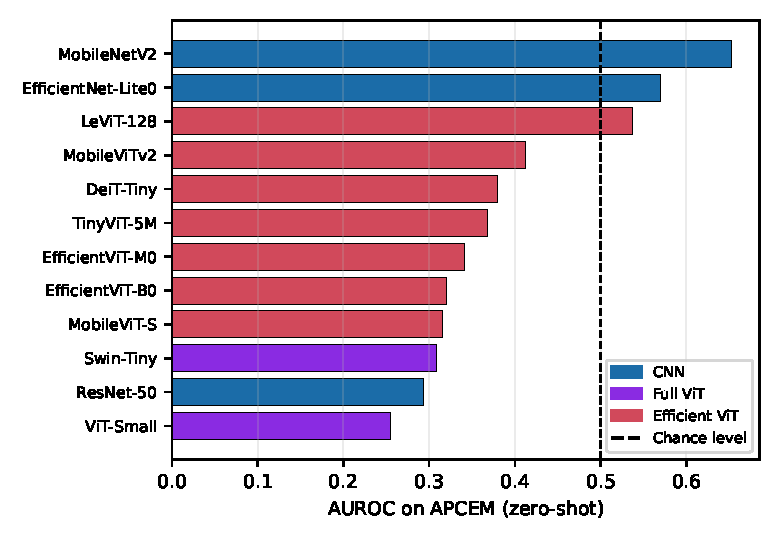
\includegraphics[width=0.82\textwidth]{figs/p1_fig3_apcem_shift.pdf}
\caption{AUROC on APCEM (zero-shot), sorted and colored by architecture family. Unlike Mendeley LBC, the CNN family spans both the best (MobileNetV2) and one of the worst (ResNet-50) models; no family-level pattern survives this third dataset.}
\label{fig:apcem-shift}
\end{figure}

\begin{figure}[htbp]
\centering
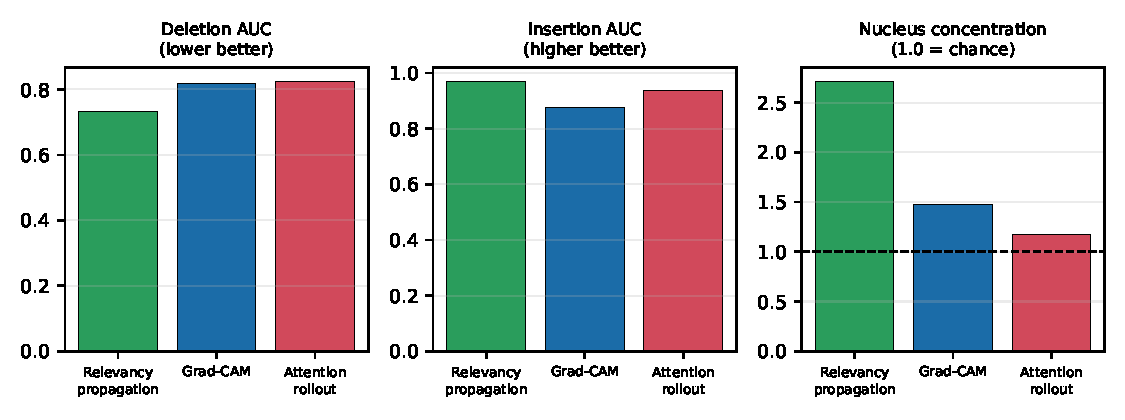
\includegraphics[width=\textwidth]{figs/p3_fig1_explainability_metrics.pdf}
\caption{Deletion AUC, insertion AUC, and nucleus concentration ratio for the three explainability methods. Relevancy propagation wins on all three, with the widest margin on nucleus concentration.}
\label{fig:xai-metrics}
\end{figure}

\begin{figure}[htbp]
\centering
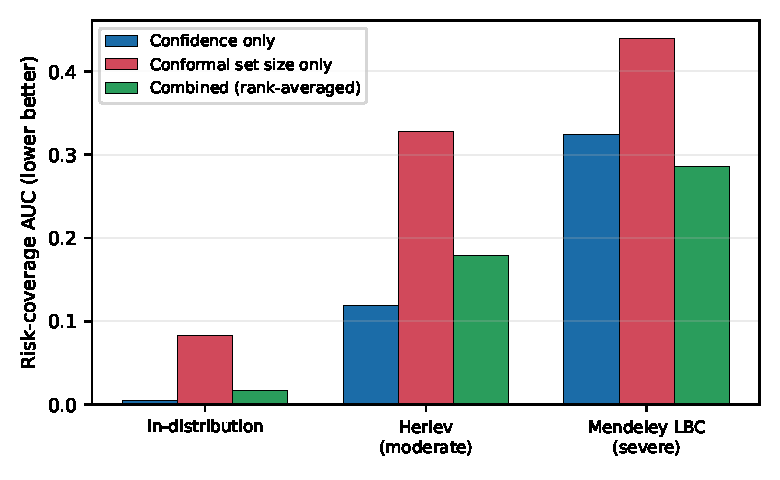
\includegraphics[width=0.85\textwidth]{figs/p3_fig3_combined_selective.pdf}
\caption{Risk-coverage AUC for confidence alone, conformal set size alone, and the rank-averaged combination at three conditions. Combining hurts in distribution and under moderate shift but helps under severe shift.}
\label{fig:combined-selective}
\end{figure}

\begin{figure}[htbp]
\centering
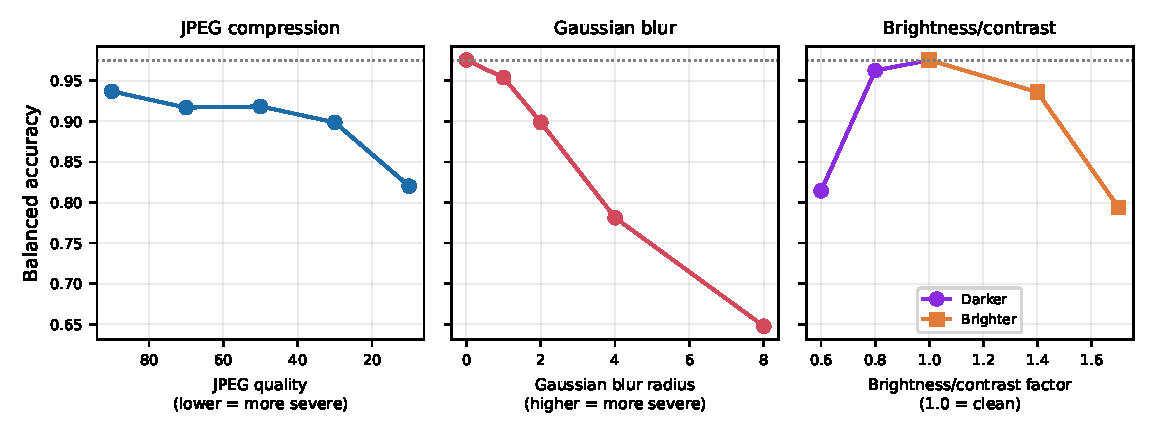
\includegraphics[width=\textwidth]{figs/p3_fig2_degradation_curves.pdf}
\caption{Balanced accuracy versus corruption severity for three synthetic degradations (EfficientViT-M0, SIPaKMeD test set). The dotted line marks the clean baseline (0.975). Gaussian blur causes the steepest decline.}
\label{fig:degradation}
\end{figure}

\begin{table}[htbp]
\centering
\caption{Class-by-class binary label mapping and image counts. NILM: negative for intraepithelial lesion or malignancy; ASC-US: atypical squamous cells of undetermined significance; ASC-H: atypical squamous cells, cannot exclude a high-grade lesion; LSIL and HSIL: low-grade and high-grade squamous intraepithelial lesion; SCC: squamous cell carcinoma. Metaplastic cells in SIPaKMeD are benign and mapped to normal; the equivocal ASC-US and ASC-H categories are grouped with abnormal, a convention that is itself debatable.}
\label{tab:labels}
\footnotesize
\begin{tabular}{@{}p{2.5cm}p{1.9cm}p{9.2cm}@{}}
\toprule
Dataset & Binary label & Original classes (images) \\
\midrule
SIPaKMeD (4,049) & Normal (2,411) & Superficial-intermediate (831), parabasal (787), metaplastic (793) \\
 & Abnormal (1,638) & Koilocytotic (825), dyskeratotic (813) \\
\addlinespace
Herlev (917) & Normal (242) & Normal columnar (98), normal intermediate (70), normal superficial (74) \\
 & Abnormal (675) & Light dysplastic (182), moderate dysplastic (146), severe dysplastic (197), carcinoma in situ (150) \\
\addlinespace
Mendeley LBC (962) & Normal (612) & NILM (612) \\
 & Abnormal (350) & LSIL (113), HSIL (163), SCC (74) \\
\addlinespace
APCEM (4,253) & Normal (779) & NILM (779) \\
 & Abnormal (3,474) & ASC-US (340), ASC-H (119), LSIL (1,241), HSIL (1,300), SSC (474) \\
\bottomrule
\end{tabular}
\end{table}

\begin{table}[htbp]
\centering
\caption{Reproducibility information. Items marked ``not recorded'' could not be recovered from the repository.}
\label{tab:repro}
\footnotesize
\begin{tabular}{@{}p{3.4cm}p{10.2cm}@{}}
\toprule
Component & Information \\
\midrule
Software versions & Cluster-grouped re-run: Python 3.13.15, torch 2.11.0+cu128, timm 1.0.29, numpy 2.1.3, CUDA 12.8, cuDNN 9.19. Original runs: minimum versions only (torch $\geq$2.2, timm $\geq$1.0); exact versions not recorded \\
Training hardware & Google Colab T4 GPU (original benchmark; other stages not individually recorded); Kaggle Tesla T4 for the cluster-grouped re-run (12 models in 1.6 GPU hours) \\
Latency hardware & One shared consumer laptop (CPU model and thread count not recorded); explanation-cost pair on a cloud virtual-machine CPU \\
Random seeds & Training seeds 13 (all stages), 17 and 29 (seed check); split seed 13 plus class index \\
Determinism & Only the PyTorch seed is set; deterministic cuDNN not enabled; NumPy, Python, and data-loader workers not separately seeded \\
Data split & One stratified cell-level manifest, identical across training seeds (main text, Sec. 3.3) \\
Checkpoint selection & Lowest validation loss, early stopping (patience 7, at most 30 epochs) \\
\bottomrule
\end{tabular}
\end{table}

\end{document}
